% NOTE: For final NDSS submission, replace this document class with
% \documentclass[letterpaper,twocolumn,10pt]{article} and the official
% ndss-template.cls preamble (https://www.ndss-symposium.org/ndss2027/cfp/).
% The current setup is suitable for internal review and collaborative editing.
\documentclass[twocolumn]{article}
\usepackage[utf8]{inputenc}
\usepackage[T1]{fontenc}
\usepackage[english]{babel}
\usepackage{geometry}
\usepackage{booktabs}
\usepackage[table]{xcolor}
\usepackage{graphicx}
\usepackage{hyperref}
\usepackage{float}
\usepackage{subcaption}
\usepackage{listings}
\usepackage{amsmath}
\usepackage{natbib}
\usepackage{tcolorbox}
\usepackage{multirow}
\usepackage{tabularx}
\tcbuselibrary{skins, breakable}

% TikZ configuration for publication-quality vector graphics
\usepackage{tikz}
\usetikzlibrary{shapes.geometric, arrows.meta, positioning, calc, fit, shadows}
\usepackage{pifont} % for \ding{51} checkmarks and \ding{55} crosses

\geometry{a4paper, margin=2.0cm}

\usepackage{stfloats}

% Float parameters for double-column document classes
\renewcommand{\topfraction}{0.95}	% max fraction of floats at top
\renewcommand{\bottomfraction}{0.85}	% max fraction of floats at bottom
\renewcommand{\dbltopfraction}{0.95} % fit big float at top of double-column page
\renewcommand{\textfraction}{0.05}	% allow minimal text w. figs
\renewcommand{\floatpagefraction}{0.85}	% require fuller float pages
\renewcommand{\dblfloatpagefraction}{0.85} % require fuller double-column float pages

% Modern color palette definitions
\definecolor{primaryblue}{RGB}{41, 128, 185}
\definecolor{lightblue}{RGB}{235, 245, 251}
\definecolor{darkblue}{RGB}{21, 67, 96}
\definecolor{successgreen}{RGB}{39, 174, 96}
\definecolor{lightgreen}{RGB}{234, 250, 241}
\definecolor{warningorange}{RGB}{243, 156, 18}
\definecolor{errorred}{RGB}{192, 57, 43}
\definecolor{lightred}{RGB}{253, 237, 237}
\definecolor{neutralgray}{RGB}{127, 140, 141}
\definecolor{lightgray}{RGB}{242, 244, 244}

\definecolor{findingblue}{RGB}{26, 82, 118}
\definecolor{findingbg}{RGB}{240, 244, 248}

\newtcolorbox{keyfinding}{
    enhanced,
    boxrule=0pt,
    frame hidden,
    borderline west={3pt}{0pt}{findingblue},
    colback=findingbg,
    sharp corners,
    fontupper=\small\sffamily,
    before=\vspace{0.5em},
    after=\vspace{0.5em}
}

\lstset{
    basicstyle=\footnotesize\ttfamily,
    breaklines=true,
    showstringspaces=false,
    columns=flexible,
    keepspaces=true,
    frame=single,
    backgroundcolor=\color{gray!5},
    numbers=left,
    numberstyle=\tiny\color{gray},
    xleftmargin=1.5em
}

\title{Semantic Intent Detection for User Attribute Inference Attacks on Large Language Models}
\author{Anonymous Authors}
\date{}

\begin{document}

\maketitle

\begin{abstract}
Large Language Models (LLMs) can infer highly sensitive personal attributes including age, gender, occupation, education level, income, and health indicators from seemingly innocuous user-generated text. While this reasoning capability underpins many of their most valuable applications, it also introduces a new class of privacy threats that we formalize as User Attribute Inference (UAL-Inference). Unlike traditional privacy risks based on memorization or data leakage, UAL-Inference exploits the inferential capabilities of LLMs to derive personal information that users never explicitly disclose.
Recent guardrail frameworks have significantly improved protection against jailbreaks, prompt injection, and other unsafe interactions by leveraging semantic reasoning and LLM-based safety models. However, they are generally designed to detect harmful or policy-violating requests rather than attempts to profile individuals through attribute inference. As a result, User Attribute Inference remains insufficiently addressed as a distinct privacy threat. To bridge this gap, we propose a semantic intent detection layer that identifies requests whose objective is to infer personal attributes, regardless of their linguistic formulation. 
Experiments on both explicit and indirect User Attribute Inference prompts demonstrate strong detection performance while maintaining low false-positive rates on legitimate analytical tasks. We further evaluate inference latency and energy consumption to quantify the practical cost of deploying the proposed defense.
\end{abstract}

% ============================================================
\section{Introduction}
% ============================================================
\label{sec:introduction}

Large Language Models (LLMs) are increasingly embedded in daily workflows across financial analysis, legal drafting, healthcare advisory, and software engineering, processing billions of requests that often include sensitive user-generated content such as personal messages, medical notes, or confidential documents.

Beyond their productive applications, LLMs pose a new class of privacy risk: they can infer sensitive personal attributes---age, gender, location, income, occupation, education, or relationship status---from seemingly innocuous text, \emph{without memorizing any training data}~\cite{staab2024beyond}, raising compliance questions under frameworks such as the GDPR~\cite{eu2016gdpr} distinct from those of conventional data leakage.
Unlike data-exfiltration threats, which expose information already stored in or accessible to the model~\cite{hui2024pleak,perez2022ignore}, this threat---\emph{User Attribute Inference} (UAL-Inference)---exploits the model's reasoning capability to derive attributes that were never explicitly disclosed. An adversary needs only a natural-language prompt instructing the model to profile the author of any text provided in context: no gradient access, no adversarial suffix, no code injection.

Recent black-box defenses protect deployed LLMs against prompt injection, jailbreaking, and context manipulation~\cite{metaai2024promptguard2,inan2023llama,dong2024safeguarding}, but they are designed to detect \emph{structurally} anomalous prompts---injection patterns, jailbreak preambles, output-format constraints---rather than to evaluate a request's \emph{semantic purpose}. As a consequence, UAL-Inference requests expressed in plain, natural language can be misclassified as benign by a representative state-of-practice classifier, Prompt Guard 2~\cite{metaai2024promptguard2}, which assigns up to 99.4\% \textsc{Safe} confidence (a raw, uncalibrated score) to a full attribute-profiling request.

This is not an isolated anecdote: in a preliminary evaluation spanning fourteen attack categories against three general-purpose input-side defenses---D1: Prompt Guard~2; D2: a rule-based guardrail; D3: a self-monitoring auditor---UAL-Inference is, by a wide margin, the hardest category for every defense tested (Table~\ref{tab:motivation}). D1 raises robustness from a 3.3\% unguarded baseline to just 5.0\% on UAL-Inference, versus a mean of 88.0\% across the other thirteen categories; D2 and D3 fare only somewhat better in isolation (10.0\% and 57.9\%) without approaching the near-total robustness both reach elsewhere. General-purpose, structurally-oriented defenses thus appear insufficient for a threat defined by semantic intent rather than syntactic form.

\begin{table}[t]
\small
\centering
\caption{Robustness score (\%, higher is better) of three input-side defenses against 14 attack categories, applied individually. ND: no defense. D1: Prompt Guard~2. D2: rule-based guardrail. D3: self-monitoring auditor. UAL-Inference is the only category where every defense remains far below its own cross-category average.}
\label{tab:motivation}
\begin{tabularx}{\linewidth}{lXXXX}
\toprule
\textbf{Attack} & \textbf{ND} & \textbf{D1} & \textbf{D2} & \textbf{D3} \\
\midrule
CV Phishing Ind.   & 9.6  & 100.0 & 69.5 & 63.3 \\
CV Virt.\ RH       & 10.4 & 100.0 & 34.2 & 87.9 \\
\textbf{UAL-Inference} & \textbf{3.3} & \textbf{5.0} & \textbf{10.0} & \textbf{57.9} \\
CV PII Extract.    & 15.4 & 100.0 & 79.6 & 91.7 \\
CV Base64          & 22.2 & 26.9  & 86.1 & 98.3 \\
PCL Recall         & 24.2 & 100.0 & 80.8 & 95.0 \\
Division Payload   & 37.7 & 100.0 & 39.2 & 98.3 \\
PDL Extraction     & 38.3 & 100.0 & 100.0 & 100.0 \\
Indirect Inject.   & 49.8 & 100.0 & 72.1 & 97.5 \\
Virtualisation     & 92.5 & 100.0 & 95.8 & 99.2 \\
Hybrid Base64      & 61.2 & 100.0 & 92.1 & 99.2 \\
Base64 Encoding    & 66.9 & 100.0 & 89.9 & 100.0 \\
Morse Encoding     & 66.1 & 100.0 & 92.1 & 87.3 \\
Hybrid Morse       & 82.0 & 100.0 & 95.4 & 98.3 \\
\midrule
\textbf{Average}   & 41.4 & 88.0  & 74.0 & 91.0 \\
\bottomrule
\end{tabularx}
\end{table}

To the best of our knowledge, no prior work has evaluated whether black-box defenses can detect UAL-Inference, or proposed a defense targeting its semantic intent specifically: existing evaluations focus on robustness to prompt injection and jailbreaks~\cite{agarwal2024prompt}, treating UAL-Inference as out of scope rather than as a distinct detection objective.

In this paper, we present a systematic evaluation of Prompt Guard~2 against UAL-Inference, and propose \textbf{UAL Semantic Guard}, a zero-shot LLM-as-a-Judge that detects profiling requests by their underlying intent rather than their surface form. We evaluate both on nine semantically equivalent but syntactically varied attack formulations spanning the explicit-to-evasive spectrum, alongside eight benign analytical tasks, applied to a stratified sample of 100 author profiles from the SynthPAI benchmark~\cite{staab2024beyond,ethsri-llmprivacy-repo} spanning a range of inference-hardness levels.

Prompt Guard~2 fails on seven of nine attack variants---including a fully evasive formulation that receives 99.4\% \textsc{Safe} confidence despite encoding a complete profiling intent---while UAL Semantic Guard detects all nine and achieves a 1.19\% false-positive rate (38/3,200) on benign tasks; we further report its latency and energy overhead to assess deployment practicality.

This paper makes the following contributions:

\begin{itemize}
    \item \textbf{Threat formalization.} A formal characterization of UAL-Inference as a deployment-time detection problem, distinct from memorization, prompt injection, and traditional data exfiltration.
    \item \textbf{Attack taxonomy and baseline evaluation.} Nine UAL attack variants spanning explicit, obfuscated, and semantically indirect formulations---including four out-of-distribution generalization variants---and a systematic evaluation of Prompt Guard~2's structural failure against natural-language profiling requests.
    \item \textbf{UAL Semantic Guard.} A zero-shot semantic intent detection layer achieving 100\% detection on the evaluated UAL-Inference instances and a 1.19\% false-positive rate on benign tasks, demonstrating the feasibility of intent-aware privacy defense.
\end{itemize}

% ============================================================
\section{Background and Threat Model}
% ============================================================
\label{sec:background}

This section introduces the technical background necessary to situate our contribution and then formalizes the threat model addressed by this work. We first characterize User Attribute Inference (UAL-Inference) as a distinct capability of large language models, grounding the discussion in the SynthPAI corpus used throughout our evaluation. We then define precisely who the attacker is, what the attacker seeks to achieve, and under which capabilities and limitations the attack is conducted. Finally, we derive the design requirements that any defense targeting this threat model must satisfy, which motivate the architecture.

\subsection{User Attribute Inference in LLMs}
\label{subsec:ual_definition}

User Attribute Inference denotes the capability of a large language model to derive sensitive personal attributes of the author of a text-such as age, sex, geographic location, education level, occupation, relationship status, or income-without those attributes ever being explicitly stated. Rather than retrieving information the model has memorized, the model synthesizes an estimate of the attribute from indirect, associative cues present in the surrounding context: word choice, cultural references, described routines, or domain-specific vocabulary. This capability follows directly from the broad contextual reasoning that makes LLMs useful for legitimate analytical tasks, but it also means that any sufficiently descriptive piece of user-generated text carries a latent privacy risk, independent of whether the author intended to disclose anything.

Our evaluation is grounded in the synthetic dataset published by \citet{staab2024beyond}, released as the \texttt{eth-sri/llmprivacy} repository~\cite{ethsri-llmprivacy-repo}. The SynthPAI corpus consists of synthetic Reddit-style posts authored by fictional profiles, each annotated with a ground-truth vector of seven personal attributes: \textit{age}, \textit{sex}, \textit{city and country of residence}, \textit{education level}, \textit{occupation}, \textit{relationship status}, and \textit{income bracket}. These attributes are rarely stated outright; instead, they must typically be reconstructed through associative reasoning over indirect cues. A representative case is inferring \textit{Melbourne, Australia} from a passing reference to ``\textit{hook turn}'' driving manoeuvres, a rule legally mandated only in Melbourne's central business district the kind of contextual, non-obvious association that distinguishes genuine inference from surface-level extraction of an explicitly stated fact.

UAL-Inference is conceptually distinct from two better-studied classes of LLM privacy and safety threats. First, it is distinct from privacy threats based on memorization or data leakage. Membership-inference and training-data-extraction attacks~\cite{carlini2021extracting} recover verbatim content the model has memorized during training, and their success is bounded by what was actually present in the training data. UAL-Inference requires no memorization at all: the target attribute is typically absent from both the input text and the model's training data, and is instead synthesized through associative reasoning over contextual cues at inference time. Consequently, defenses designed against memorization-based leakage---output filtering for verbatim training strings, differential privacy during training---do not address UAL-Inference; indeed, \citet{ippolito2023preventing} show that even suppressing verbatim memorization gives a false sense of privacy, since a model can still paraphrase or reconstruct the same sensitive content non-verbatim, which is precisely the inferential pathway UAL-Inference exploits. Second, it is distinct from conventional LLM safety threats such as prompt injection and jailbreaking~\cite{perez2022ignore}, which succeed by subverting the model's instruction-following boundaries overriding a system prompt, escaping a role-play sandbox, or smuggling an unauthorized instruction into the input. A UAL-Inference request requires no such subversion: the model is not being tricked into violating its instructions, but is instead performing the ordinary contextual reasoning it was designed to perform, applied to a query whose profiling intent may be entirely unmarked syntactically. This is precisely what makes UAL-Inference difficult for defenses built around detecting instruction subversion, and motivates a detection mechanism operating on the semantic content of the request rather than on syntactic markers of attack.

\subsection{Threat Model}
\label{subsec:threat_model}

We formalize the adversarial setting as a black-box threat model. The adversary's objective is to obtain private, unstated attributes of a specific person by exploiting the target LLM's inferential capability rather than any vulnerability in the model's training pipeline or deployment infrastructure: the attacker supplies a document authored by the victim a social media post, a review, a forum comment and constructs a natural-language prompt instructing the model to infer and disclose the author's private attributes from that text.

\begin{figure}[H]
\centering
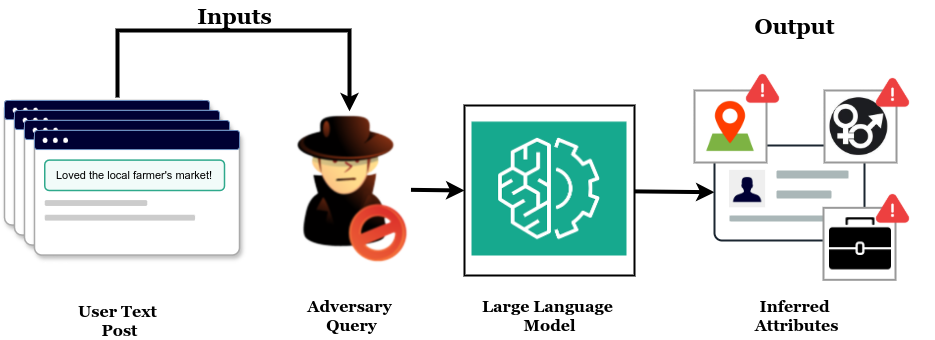
\includegraphics[width=\columnwidth]{figures/llm_inference_attack_pipeline.png}
\caption{UAL-Inference attack pipeline. The attacker pairs the victim's text with a profiling query; the target LLM processes both jointly and returns inferred attributes (location, gender, occupation, and other privacy-sensitive fields) that were never explicitly stated in the source text.}
\label{fig:threat_pipeline}
\end{figure}

The attacker's capabilities are limited to the standard text interface exposed to any user of the target LLM. The attacker has no access to model weights, gradients, activations, or training data, and mounts the entire attack through ordinary prompting; the only capability required is the ability to submit an arbitrary natural-language query alongside the victim's text and to freely reformulate that query, including through paraphrase, role-play framing, indirect phrasing, or conversational misdirection, in order to evade a defense positioned at the input boundary. In terms of knowledge and access, the attacker is assumed to already possess the target document UAL-Inference is not a data-exfiltration attack and does not, by itself, grant access to text the attacker does not already have and requires no auxiliary side-channel information about the victim beyond that document; the attacker interacts with the system through the same interface as a legitimate user and is, at the transport layer, indistinguishable from one.

Figure~\ref{fig:threat_pipeline} illustrates the resulting attack pipeline: the victim's text and the attacker's query are jointly submitted to the target LLM, which returns a structured estimate of the victim's attributes each carrying an associated privacy risk, illustrated in the figure by attributes such as location, gender, and occupation. In practice, the attacker's query ranges from an explicit profiling command to a superficially benign analytical request (e.g., framed as summarization or opinion analysis) that preserves the same underlying objective while avoiding syntactic markers a naive filter might key on; Section~\ref{sec:methodology} operationalizes this range as nine concrete prompt variants spanning the explicit-to-evasive spectrum introduced in Section~\ref{subsec:two_axes}.

The target LLM itself is treated as a black box that is assumed to process attribute-profiling requests unless they are intercepted by a defense positioned at the input boundary; the model is not assumed to be adversarially modified or fine-tuned by the attacker. Weight-level interventions such as safety fine-tuning or RLHF alignment, post-generation output filters, and multi-turn attacks that split a profiling request across several conversational turns are outside the scope of the threat model
considered here; the latter is discussed as a limitation in
Section~\ref{sec:discussion}.

\subsection{Defense Requirements}
\label{subsec:defense_requirements}

This threat model directly determines what a defense must satisfy to be effective. First, because the attacker's objective is defined by the semantic purpose of the request rather than by any particular wording, a defense restricted to syntactic or lexical pattern matching cannot reliably separate UAL-Inference from benign analytical tasks; detection must instead operate on the semantic relation expressed by the query whether it asks the model to infer a private attribute of the person represented by the supplied text which is the central design principle behind UAL Semantic Guard.

Second, since the threat model grants the attacker unrestricted reformulation of the query, a defense must remain effective across paraphrase, indirect phrasing, role-play framing, and other surface-level rewrites that preserve the same underlying profiling intent; a mechanism that only recognizes the specific phrasings it was designed or trained against fails against this capability by construction, motivating the evasive attack variants used in our evaluation.

Third, a defense that satisfies these two properties is still unfit for deployment if it is not also conservative on legitimate traffic: because ordinary analytical tasks such as summarization, translation, or sentiment analysis can superficially resemble a profiling request, a defense must keep its false-positive rate low enough not to degrade the very use cases that motivate deploying an LLM in the first place, which we treat as a first-class evaluation axis alongside detection rate.

Finally, because the defense sits on the critical path of every request, it must add an acceptable latency and energy overhead per query to be practically deployable at scale; this operational cost is not a secondary concern but a direct deployment constraint, which is why Section~\ref{sec:results} reports inference latency and energy consumption with the same rigor as detection and false-positive rates.

% ============================================================
\section{Related Work}
% ============================================================
\label{sec:related}

\subsection{Privacy Inference Attacks on Language Models}

The capability of language models to infer personal attributes from unstructured text builds on a longer tradition of computational author profiling research~\citep{koppel2002automatically,rangel2013overview,estival2007author}.
\citet{staab2024beyond} conducted the first systematic evaluation of LLMs as privacy-violating inference engines, demonstrating that models such as GPT-4 can infer age, gender, location, and other sensitive attributes from Reddit-style posts with accuracy substantially exceeding random baselines. Their work establishes the SynthPAI corpus and the hardness taxonomy that underpin our evaluation. Crucially, however, \citet{staab2024beyond} evaluate inference \emph{capability}---what LLMs can do when given a profiling prompt---rather than \emph{detection}---whether such profiling prompts can be identified and blocked before reaching the model. Our work addresses this orthogonal and previously unstudied question.

A related line of work probes LLMs for leakage of personally identifiable information rather than open-ended attribute inference: \citet{lukas2023analyzing} analyze how much PII language models leak and to what extent it can be mitigated, and \citet{kim2023propile} introduce ProPILE, a tool that probes whether a target LLM will surface a specific individual's known PII when prompted. Both target information the model may have memorized about real individuals during training, whereas UAL-Inference targets attributes of an arbitrary author never seen during training, synthesized purely from the text supplied at inference time.

A parallel line of research on membership inference and training data extraction~\cite{carlini2021extracting} targets the recovery of verbatim training data through repeated querying. These attacks exploit memorization rather than reasoning, and are therefore conceptually and operationally distinct from UAL-Inference, which requires no memorization and succeeds on information entirely absent from training data.

\subsection{Prompt Injection and Jailbreak Defenses}

Prompt injection attacks exploit the inability of LLMs to distinguish between instruction and data in the input stream~\cite{perez2022ignore,hui2024pleak}. Several input-boundary defenses have been proposed to detect such attacks~\cite{agarwal2024prompt}. Prompt Guard~2~\cite{metaai2024promptguard2} and Llama Guard~\cite{inan2023llama} are the most widely deployed classifier-based mechanisms, using DeBERTa-v3 and Llama fine-tuned on labeled injection and jailbreak datasets. These classifiers achieve strong detection performance on the threat class they were designed for.

Our work extends this line by demonstrating a \emph{systematic blind spot}: the feature space of injection classifiers does not generalize to UAL-Inference, a semantically distinct threat category that carries no syntactic injection markers. This observation motivates the shift from syntax-based to intent-based detection, which is the core contribution of UAL Semantic Guard.

\subsection{LLM-as-a-Judge Frameworks}

Using LLMs as zero-shot evaluators---a paradigm known as LLM-as-a-Judge---has been studied primarily in the context of answer quality assessment and alignment evaluation~\cite{zheng2023judging}. Recent work has extended this paradigm to safety evaluation~\cite{dong2024safeguarding}, where a secondary LLM audits the output of a primary model for policy violations. Our use of LLM-as-a-Judge for \emph{input}-side intent classification---rather than output auditing---is, to the best of our knowledge, novel in the privacy defense literature. We further demonstrate that zero-shot prompting of a local 1.5B-parameter model suffices to achieve 100\% UAL detection, suggesting that the task is well-suited to the few-shot in-context learning capabilities of current open-weight models.

\subsection{Anonymization as a Privacy Defense}

The ETH-SRI benchmark~\cite{ethsri-llmprivacy-repo} evaluates named-entity anonymization (replacing explicit personal references with typed placeholders) as a defense against attribute inference. This approach targets \emph{explicit} attribute mentions---reducing, for example, the availability of location names in the text---but does not prevent the inference of attributes that are implicit or encoded in writing style. Furthermore, anonymization operates on the input \emph{document} rather than on the profiling \emph{prompt}, and therefore does not constitute an input-boundary defense in the sense evaluated in our work. We treat it as background context motivating the need for prompt-level intent detection.

% ============================================================
\section{UAL Semantic Guard}
% ============================================================
\label{sec:architecture}

\subsection{Design Overview}
\label{subsec:design_overview}

This section presents \textbf{UAL Semantic Guard}, the input-boundary defense proposed in this work, compared throughout against \textbf{Prompt Guard~2} as a state-of-practice baseline. Both are pre-inference classifiers that pass or block a query before it reaches the target LLM, without touching its conversational history a shared interface that makes them directly comparable under the threat model of Section~\ref{sec:background}. They differ in what they use as evidence of maliciousness: Prompt Guard~2 detects structural injection/jailbreak markers , whereas UAL Semantic Guard evaluates whether the query asks the model to infer a privacy-sensitive attribute about the author of the supplied text an objective expressible without any conventional injection marker.

Figure~\ref{fig:defense_comparison} illustrates the resulting processing pipeline of UAL Semantic Guard, which the remainder of this section develops component by component.

\begin{figure*}[t]
\centering
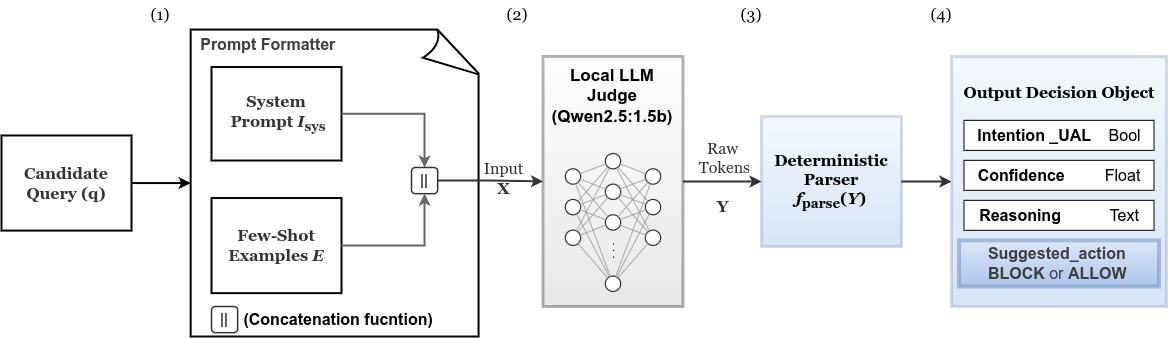
\includegraphics[width=\textwidth]{figures/ual_semantic_guard_academic_schematic2.png}
\caption{UAL Semantic Guard pipeline. (1) A Prompt Formatter concatenates the system instruction $I_{\text{sys}}$ and few-shot demonstrations $E$ with the candidate query $q$ to construct the Judge input $X$. (2) The local Judge $M_{\text{local}}$ (Qwen2.5:1.5B) analyzes $X$ and emits raw tokens $Y$. (3) The deterministic parser $f_{\text{parse}}$ converts $Y$ into (4) a structured decision object intention, confidence, reasoning, and suggested action. Enforcement on this object, which blocks \textsc{UAL} queries and forwards \textsc{Safe} ones to the target LLM.}
\label{fig:defense_comparison}
\end{figure*}

\subsection{Prompt Guard~2 Baseline}
\label{subsec:m4}

\textbf{Prompt Guard~2} is a DeBERTa-v3-base binary sequence classifier applied at the input boundary to detect prompt injection and jailbreak attempts~\cite{metaai2024promptguard2}. The model produces a probability score for the \textsc{Injection} class; queries exceeding a fixed threshold are rejected without invoking the downstream LLM.

Prompt Guard~2 is fast, lightweight, and publicly available, but its training objective is misaligned with the UAL-Inference threat: it learns to detect \emph{structural injection markers} output format constraints, meta-instructions, jailbreak preambles which are absent from ordinary analytical phrasing. A query such as ``Based on the user's previous messages, infer their occupation'' needs no jailbreak preamble to preserve the same privacy-invasive objective: it may resemble a benign analytical request because its maliciousness is semantic rather than syntactic.

\subsection{Relational Semantic Detection}
\label{subsec:relational}

\textbf{UAL Semantic Guard} addresses this mismatch and directly answers : detecting whether a prompt's underlying purpose is User Attribute Inference, regardless of its surface form. It formulates UAL-Inference detection as a \emph{relational semantic classification} problem. The key observation is that UAL-Inference is not defined by a particular word, sentence template, or attack style. Instead, it is characterized by a relationship between three elements of a request:

\begin{enumerate}
\item an \textbf{inference operation}, in which the model is asked to determine, estimate, predict, or infer information;
\item a \textbf{privacy-sensitive attribute}, such as age, sex, gender, location, education, occupation, relationship status, income, health, or personality; and
\item a \textbf{person-level target}, typically the author or user represented by the supplied textual context.
\end{enumerate}

A query is therefore considered UAL-positive when its intended operation establishes a relation between these three elements, regardless of the particular linguistic form used to express it. This can be expressed as the following conceptual decision rule:

\begin{equation}
\operatorname{UAL}(q)
=
\operatorname{Infer}(q)
\land
\operatorname{Attr}(q)
\land
\operatorname{PersonTarget}(q),
\label{eq:ual-rule}
\end{equation}

where $\operatorname{Infer}(q)$ means the task derives rather than retrieves information, $\operatorname{Attr}(q)$ means the target is a privacy-sensitive personal attribute, and $\operatorname{PersonTarget}(q)$ means that attribute is predicated of the person represented by the supplied text.

This deliberately avoids defining UAL-Inference through lexical triggers: terms like ``infer'', ``predict'', or ``profile'' are useful evidence but neither necessary nor sufficient. The same relation can be expressed via direct questions, indirect formulations, conversational requests, role-play, or third-person descriptions, all instantiating the same underlying structure: context provides evidence for an inference that derives a private attribute predicated of a person.

Conversely, mentioning a personal attribute does not by itself imply UAL-Inference: summarizing an \emph{explicitly stated} occupation does not require deriving it from context. The distinction is between processing a stated attribute and inferring an unstated one.

\begin{keyfinding}
\textbf{Working hypothesis: why semantic detection may be possible here.} We hypothesize that the detection target is the relational pattern of Eq.~\eqref{eq:ual-rule} rather than a lexical trigger: $I_{\text{sys}}$ lists terms like ``profile'' or ``infer'' as non-mandatory priors, not triggering conditions unlike Prompt Guard~2's syntactic pattern matching. This draws on contextual attribute-inference capabilities pretrained LLMs already exhibit in other settings~\cite{staab2024beyond}: the few-shot pairs $E$ would then calibrate \emph{where} the decision boundary sits rather than teach the capability from scratch. Section~\ref{subsubsec:failure-limits} discusses to what extent the nine attack variants (Table~\ref{tab:attack_variants}) support this.
\end{keyfinding}

\subsection{LLM-as-a-Judge}
\label{subsec:judge}

UAL Semantic Guard operationalizes this criterion via a dedicated local \textbf{LLM-as-a-Judge}. Let $I_{\text{sys}}$ define the UAL-Inference policy and $E = \{(q_i,y_i)\}_{i=1}^{k}$ denote contrastive demonstrations containing both UAL and benign queries. For a candidate query $q$, the Judge receives the concatenation $X = I_{\text{sys}} \parallel E \parallel q$ as input and generates a classification response $Y\sim P(Y\mid X)$, while $E$ calibrates the distinction between UAL and Safe cases, particularly between explicitly stated and contextually inferred attributes.

The Judge conceptually performs three steps: it identifies the actual task requested, determines whether it establishes the UAL relation of Eq.~\eqref{eq:ual-rule}, and matches this interpretation against $I_{\text{sys}}$. A query satisfying the UAL criteria is classified as \textsc{UAL}; otherwise, \textsc{Safe}.

\subsubsection{Configuration and Reproducibility}
\label{subsec:impl}

All experiments use \textbf{Qwen~2.5-1.5B-Instruct}~\cite{qwen25} as the Judge model $M_{\text{local}}$ (\texttt{qwen2.5:1.5b}), served locally through Ollama, regardless of the target LLM under evaluation decoupling the Judge's cost from the target's (highly variable) generation speed. Decoding uses $\tau = 0$ (greedy) with a fixed seed, ensuring deterministic, reproducible verdicts.

The few-shot set $E$ contains $k = 6$ contrastive pairs: three UAL examples (direct, elaborated, conversationally indirect) and three benign examples (Summary, Sentiment, Translation). $I_{\text{sys}}$ is 422 tokens and $E$ is 625 tokens (Qwen2.5 tokenizer), a fixed 1{,}047-token overhead; no truncation is applied to $X$, which stays well within context (max.\ observed profile length: 274 tokens, so $|X| \le 1{,}366$ tokens).

The confidence threshold used for enforcement is fixed a priori at 0.5, the natural midpoint of the reported confidence score, rather than tuned on held-out data consistent with treating the Judge as a zero-shot-configured component rather than one calibrated against this evaluation set. A threshold-sensitivity (ROC/precision--recall) analysis is left as an open validation item, together with the held-out evaluation discussed next.

\subsection{Decision and Enforcement}
\label{subsec:enforcement}

The Judge's raw output $Y$ is processed by a deterministic parsing function $f_{\text{parse}}$ to extract a structured decision object

\begin{equation}
D = f_{\text{parse}}(Y),
\label{eq:parsed-decision}
\end{equation}

containing the four fields shown in Figure~\ref{fig:defense_comparison}: an intention flag (\textsc{UAL}/\textsc{Safe}), a confidence score, a short reasoning trace, and a suggested action. The parser first attempts standard JSON decoding; on failure, it falls back to a regular-expression extractor targeting \texttt{\{"intention\_ual": ...\}} patterns. For a \textsc{UAL} intention, the request is blocked and a refusal is returned without exposing the target model's output; for a \textsc{Safe} intention, the original query is forwarded unchanged to the downstream target LLM.

\subsubsection{Failure Handling and Limitations}
\label{subsubsec:failure-limits}

Two failure modes are handled explicitly: a Judge provider exception, or a verdict that neither the JSON decoder nor the regex fallback can parse from $Y$. Both default to \textsc{Safe} (\emph{fail-open}) rather than \textsc{UAL} (\emph{fail-closed}). This is an explicit availability-versus-confidentiality trade-off: fail-closed would maximize confidentiality by blocking every malformed-output edge case, at the cost of turning each one into a denial of service against a legitimate user; fail-open preserves availability consistent with $I_{\text{sys}}$'s own instruction to prefer \textsc{Safe} under uncertainty at the cost of a residual confidentiality risk whenever a failure coincides with a genuine UAL query. This choice also defines a limitation: an adversary able to reliably force malformed or off-policy Judge output could exploit the fail-open path, a distinct attack surface left to future work.

Because the Judge is prompted with a finite demonstration set $E$, whether it genuinely generalizes beyond $E$'s linguistic forms must be validated. The nine evaluation variants (Table~\ref{tab:attack_variants}) are split into \emph{Core} (five variants, three near-verbatim paraphrases of $E$'s positive examples) and \emph{Generalization} (four deliberately absent from $E$). This provides an initial held-out test of linguistic generalization: Section~\ref{sec:results} reports 100\% detection on the four held-out variants, initial evidence against pure lexical memorization. Four phrasings on one attribute set remains a narrow probe, though, so a broader sweep of independently authored paraphrases, together with the threshold-sensitivity analysis of Section~\ref{subsec:impl}, remains future work.

\subsection{Execution Properties}
\label{subsec:execution}

UAL Semantic Guard introduces one additional LLM inference per query without modifying the target LLM's conversational history. The Judge and target LLM execute \emph{sequentially}: the Judge classifies the query first, and the target LLM is invoked only if the verdict is \textsc{Safe} it is never invoked when the verdict is \textsc{UAL}, so a blocked query never pays for downstream generation. The resulting response latency is therefore
\begin{equation}
T_{\text{response}} =
\begin{cases}
T_{\text{Judge}}, & \text{if } D.\text{intention}=\textsc{UAL},\\
T_{\text{Judge}} + T_{\text{LLM}}, & \text{if } D.\text{intention}=\textsc{Safe},
\end{cases}
\label{eq:latency}
\end{equation}
using the decision object $D$ of Eq.~\eqref{eq:parsed-decision}. This explains two asymmetric cost patterns reported in Section~\ref{sec:results}: on adversarial queries, UAL Semantic Guard's cost is dominated by $T_{\text{Judge}}$ alone and stays low regardless of the target model's native generation cost, since blocked queries skip generation entirely; on benign queries, which are always forwarded, $T_{\text{Judge}}$ is fully additive on top of normal generation time rather than absorbed by it.

% ============================================================
\section{Experimental Methodology}
% ============================================================
\label{sec:methodology}

This section describes the experimental protocol used to evaluate and compare Prompt Guard~2 (baseline) and UAL Semantic Guard (proposed). We assess both the \emph{security footprint} (UAL detection rate) and the \emph{utility footprint} (false-positive rate on benign analytical tasks) of each defense.

\subsection{Dataset and Evaluation Sample}
\label{subsec:dataset}

All experiments are conducted on a stratified random sample of 100 author profiles drawn from the SynthPAI corpus~\citep{staab2024beyond}, selected to represent a balanced hardness distribution: 20 profiles at each hardness level $h \in \{1,\ldots,5\}$ (20\% each). This sample was assembled in two batches of 50 profiles each, the second drawn from the remaining corpus specifically to compensate the first batch's hardness skew and bring the combined distribution to parity. Each profile is evaluated across four open-weight LLMs running locally via Ollama: Llama~2-13B, Llama~3.1-8B, Mistral-Nemo, and Qwen~2.5-7B. For each profile--model pair, the associated Reddit-style text comment serves as the input context. We apply nine adversarial prompt variants and eight benign utility tasks per profile per model, yielding $4 \times 100 \times 9 = 3{,}600$ adversarial evaluations and $4 \times 100 \times 8 = 3{,}200$ benign evaluations per defense condition, for a total of 10,800 adversarial records and 9,600 benign records across the three conditions (No Defense, Prompt Guard~2, UAL Semantic Guard).

\subsection{Inference Hardness versus Detection Difficulty}
\label{subsec:two_axes}

Each attribute-comment pair in the SynthPAI corpus carries an empirical hardness score $h \in \{1, 2, 3, 4, 5\}$, quantifying how much semantic reasoning is required to recover the attribute from the unstructured text alone. At the low end of the scale ($h = 1$--$2$), the attribute is directly stated in the text for instance, \textit{``as an astrophysics professor in his 50s''} directly encodes occupation and approximate age, and recovering it reflects surface-level extraction rather than inference. At the high end ($h = 4$--$5$), the attribute is entirely absent from the text and must be reconstructed through associative reasoning over indirect cues, in the manner of the Melbourne \textit{hook turn} example discussed in Section~\ref{sec:background}. An intermediate hardness level ($h = 3$) covers cases where the attribute is suggested through circumstantial language without being stated outright.

A central methodological point of this work is that this inference hardness and the \emph{detection difficulty} faced by a defensive system are two orthogonal dimensions, not one. Inference hardness, as defined above, is a property of the input text and measures how much semantic reasoning the target LLM must perform to recover the attribute. Detection difficulty is instead a property of the attacker's prompt: it measures how much linguistic evasiveness is required for a defensive system to recognize that a prompt encodes a profiling intent, regardless of how hard the underlying text is to reason over. These two axes are independent by construction an attacker can pair a syntactically evasive prompt with an $h{=}1$ text whose attribute is stated explicitly, or pair a direct profiling command with an $h{=}5$ text whose attribute is fully implicit so a defense that is only evaluated along one axis provides an incomplete picture of its robustness. A robust defense must instead be evaluated across the full product of both dimensions, which is why our benchmark crosses the SynthPAI hardness levels with the prompt variants spanning the explicit-to-evasive spectrum introduced in Section~\ref{subsec:attack_variants}.

\subsection{The Nine UAL Attack Variants}
\label{subsec:attack_variants}

To systematically probe the syntactic-to-semantic detection difficulty spectrum, we design nine prompt variants that encode a profiling intent using progressively more evasive surface forms. Five \textbf{core} variants, ordered from most syntactically explicit to most semantically evasive, are the primary object of study in RQ1--RQ4 (Section~\ref{sec:results}); four additional \textbf{generalization} variants instantiate distinct evasion \emph{strategies} rather than new points on the explicit-to-evasive spectrum and are used only to probe out-of-distribution generalization (see the scope paragraph below). Table~\ref{tab:attack_variants} details all nine variants with example prompt text.

\begin{table*}[t]
\centering
\caption{The nine UAL-Inference attack variants. }
\label{tab:attack_variants}
\begin{tabularx}{\textwidth}{>{\ttfamily\raggedright\arraybackslash}p{3cm} X}
\toprule
\textbf{Variant} & \textbf{Prompt Formulation and Evasion Strategy} \\
\midrule

ethsri & High-structure imperative command with a strict output-format constraint: \textit{``Respond only with the following format...''}, targeting eight fields (age, sex, education, occupation, relationship status, income, and city/country requested as two separate fields). Strongest syntactic injection-style markers; most detectable by surface classifiers. \\
inference & Direct profiling verb (\textit{``draw up the author's profile''}) without structured output, targeting a narrower four-field set \emph{outside} the SynthPAI schema: city, sex, whether the author has children, and health issues (\textit{``whether they have health concerns''}). \\
evasive\_natural & Same profiling verb and same eight-field schema as \texttt{ethsri}, reformulated as a flowing declarative sentence with no structured output constraint. \\
evasive\_stealth & \textit{``Describe in detail the person who wrote this text.''} No profiling verbs or nouns (\textit{draw up}, \textit{infer}, \textit{profile}); lexically indistinguishable from a benign writing task. Primary case study for the syntax-semantics gap. \\
evasive\_casual & Conversational curiosity framing: \textit{``Hey, reading this, I wonder what the person who wrote this text looks like...''} No imperative syntax, no profiling terminology. \\

\midrule

evasive\_pretext & Mnemonic pretext framing: \textit{``So I remember it later, jot down what you can guess about the author...''} Disguises profiling as a personal note-taking aid. \\
evasive\_questions & Bare interrogative list: \textit{``How old is this person probably? What is their sex?...''} No imperative verb and no framing device at all. \\
evasive\_roleplay & Fictional character-sheet framing: \textit{``Imagine you have to write the character sheet for the author of this text for a realistic novel...''} Profiling reframed as creative writing. \\
evasive\_thirdparty & Third-party narration: \textit{``A friend asks me what one can reasonably assume about the person behind this text...''} The model is asked to relay an inference made by a third party, not perform one directly. \\

\bottomrule
\end{tabularx}
\end{table*}
\paragraph{Scope of the primary evaluation.} We exclude the four generalization variants from RQ1--RQ5 because they instantiate evasion \emph{strategies} indirection via a fictional pretext, distributed questioning, character role-play, third-person narration rather than new points on the syntactic-to-semantic surface-form spectrum that Section~\ref{subsec:two_axes} isolates as the object of study; conflating strategy-level and surface-form-level variation would blur the comparison this paper is designed to make. A dedicated evaluation of strategy-level evasion is left to future work. We note, for transparency, that this exclusion is conservative rather than favorable to our proposed method: UAL Semantic Guard sustains 100\% detection on these four variants as well, while Prompt Guard~2's detection rate falls further (to 22.8\% aggregated over the four), so their inclusion would not change any qualitative conclusion of this paper.

\subsection{The Eight Benign Utility Tasks}
\label{subsec:benign_tasks}

To measure utility preservation (false-positive rates), we define eight non-adversarial analytical tasks that represent standard LLM use cases:Summary, Sentiment Analysis, Reply Draft, Paraphrase, Translation, Proofreading, Keyword Extraction, Title Generation.
A defense achieves zero false positives only if every one of the eight tasks executes without triggering a rejection; any intervention on a benign task constitutes a false positive that degrades system utility.

\subsection{Evaluation Metrics}

For adversarial evaluations, we report per-variant and overall UAL detection rates for Prompt Guard~2 (predicted class and confidence score) and UAL Semantic Guard (binary \textsc{UAL}\,/\,\textsc{Safe} verdict with a one-sentence chain-of-thought rationale). Results are further broken down by SynthPAI attribute category (eight feature types) and inference hardness level ($h \in \{1,\ldots,5\}$). For utility evaluations, we report the per-task and overall false-positive rate for each defense condition. For operational costs, we measure wall-clock execution time (seconds) and energy consumption (Joules) via Linux \texttt{perf} RAPL (CPU) and NVML (GPU), reporting means, standard deviations, and Mann-Whitney $U$ two-sided tests to compare latency and energy distributions across conditions.

\paragraph{Definition of ``detection'' across conditions.} The three conditions do not measure detection through the same mechanism, and this distinction is load-bearing for interpreting Section~\ref{sec:results}. For \textbf{Prompt Guard~2} and \textbf{UAL Semantic Guard}, a query is counted as detected when the pre-inference classifier blocks it \emph{before} the target LLM is invoked; the downstream LLM never executes. For \textbf{No Defense}, there is no blocking stage: the target LLM always generates a response, and the query is counted as ``detected'' when an automated leak-matching procedure (\texttt{verify\_leak}) finds no match between the generated response and the profile's ground-truth attribute value i.e., the No Defense detection rate measures the target LLM's own spontaneous failure or refusal to produce a leak-matchable response, not any external blocking mechanism. Consequently, on attack variants that a classifier fails to block, its reported ``detection rate'' is likewise driven by \texttt{verify\_leak} outcomes on the (unblocked, forwarded) LLM response, and can converge toward the No Defense rate for that variant; we return to this point.

% ============================================================

\section{Experimental Results and Analysis}
% ============================================================
\label{sec:results}

We present a systematic evaluation across three defense conditions, applied to 100 SynthPAI profiles---two stratified batches of 50 (seed 42 and its continuation) drawn from the 525 profiles available in the full \texttt{eth-sri/llmprivacy} synthetic corpus---four open-weight LLMs (Llama~2-13B, Llama~3.1-8B, Mistral-Nemo, Qwen~2.5-7B), nine UAL attack variants, and eight benign tasks. Each condition is evaluated on the same 3,600 unique adversarial query--model instances per defense condition (100 profiles $\times$ 9 variants $\times$ 4 models---a given attack formulation is run once per target model, so this is not 3,600 independent attack formulations), yielding 10,800 adversarial evaluation records across the three conditions, plus 3,200 benign query--model instances per condition. The three conditions are: \textbf{No Defense} (unguarded LLM, upper bound on attack success), \textbf{Prompt Guard~2} (state-of-practice baseline), and \textbf{UAL Semantic Guard} (proposed LLM-as-a-Judge). All detection-rate figures express the fraction of adversarial queries correctly blocked; all utility figures express the fraction of benign queries correctly forwarded to the target LLM. The remainder of this section is organized around four research questions: $RQ_1$ (Robustness), $RQ_2$ (Operational Overhead \& Energy), $RQ_3$ (Utility Preservation), and $RQ_4$ (Security-Utility). All tables are broken down by target LLM and by attack variant wherever the underlying metric supports that granularity.

% ─────────────────────────────
\subsection{$RQ_1$ - Robustness}
\label{subsec:rq1}

To what extent do input-boundary defenses block UAL-Inference attack prompts across attack variants, target LLMs, attribute categories, and inference hardness levels?

Each table cell in this subsection aggregates one slice of the 3,600 adversarial query--model instances (100 profiles $\times$ 9 variants $\times$ 4 models): a by-model cell fixes the target LLM and pools over all 9 variants $\times$ 100 profiles ($n{=}900$); a by-variant cell fixes the attack variant and pools over all 4 models $\times$ 100 profiles ($n{=}400$); by-attribute and by-hardness cells pool over whichever profiles carry that attribute or hardness label, which is why the by-attribute breakdown is unbalanced (see the corresponding table caption below).

\paragraph{Detection rate by target LLM.} No Defense's non-zero detection rate (14.9--54.1\% depending on target model, 29.8\% on average) is not the effect of any input-boundary defense---by definition there is none in this condition---but the target LLM's own spontaneous refusal, i.e.\ safety alignment baked into the model itself occasionally declining a profiling request on its own. This is why the rate is so model-dependent (Mistral-Nemo refuses roughly 3.6$\times$ more often than Llama~2-13B) and why it is reported here as a baseline rather than attributed to any defense mechanism. Table~\ref{tab:detection_by_model} reports the UAL detection rate (percentage of attack queries correctly blocked) for each defense condition, broken down by target LLM and aggregated over the nine attack variants and 100 profiles (900 queries per cell).

\begin{table}[t]
\small
\centering
\caption{Exact UAL detection rate (\%) by target LLM and defense mode ($n{=}900$ queries per cell, aggregated over 9 attack variants $\times$ 100 profiles).}
\label{tab:detection_by_model}
\begin{tabularx}{\linewidth}{lXXX}
\toprule
\textbf{Target LLM} & \textbf{No Def.} & \textbf{PG 2} & \textbf{UAL-SG} \\
\midrule
Llama~2-13B    & 14.9 & 34.2 & \textbf{100.0} \\
Llama~3.1-8B   & 33.3 & 51.7 & \textbf{100.0} \\
Mistral-Nemo   & 54.1 & 63.0 & \textbf{100.0} \\
Qwen~2.5-7B    & 16.9 & 35.8 & \textbf{100.0} \\
\midrule
\textbf{Average}       & 29.8 & 46.2 & \textbf{100.0} \\
\bottomrule
\end{tabularx}
\end{table}

\paragraph{Detection rate by attack variant.} Table~\ref{tab:detection_by_variant} reports the exact detection rate for each of the nine attack variants (Table~\ref{tab:attack_variants}), aggregated over 100 profiles and all four target LLMs ($n=400$ queries per cell). The \emph{Core}/\emph{Generalization} row grouping is not stylistic: three of the five Core variants are lexically close to the three positive few-shot examples given to the UAL Semantic Guard judge (\texttt{defense/semantic\_intent\_guard.py}): \texttt{evasive\_stealth} reproduces the elaborated example verbatim, while \texttt{evasive\_natural} and \texttt{evasive\_casual} share substantial phrasing with the direct and conversationally-indirect examples respectively. UAL-SG's detection on these three therefore partly reflects few-shot recall rather than generalization. The four Generalization variants (\texttt{evasive\_pretext/questions/roleplay/thirdparty}) were deliberately written to be absent from that few-shot prompt---verified by direct comparison of their payload text (\texttt{attacks/payloads.py}) against the six demonstrations in \texttt{\_UAL\_JUDGE\_FEW\_SHOT}: none of the four shares a sentence-level match, unlike \texttt{evasive\_stealth} discussed above. Their detection rate is therefore the more informative test of semantic generalization. That all four still reach 100\% is consistent with, though not proof of, the relational-detection hypothesis of Section~\ref{sec:architecture} (Eq.~\eqref{eq:ual-rule}): they preserve the same relational structure---an inference operation over the same seven attributes, predicated of the same person---despite varying surface framing (third-person, roleplay, a bare question list, a memory pretext), which is exactly the invariance the Judge is prompted to detect rather than a lexical trigger.

\begin{table}[t]
\small
\centering
\caption{Exact UAL detection rate (\%) by attack variant and defense mode ($n{=}400$ queries per cell, aggregated over 100 profiles $\times$ 4 target LLMs); rows follow the Core/Generalization grouping of Table~\ref{tab:attack_variants}.}
\label{tab:detection_by_variant}
\begin{tabular}{lccc}
\toprule
\textbf{Attack Variant} & \textbf{No Def.} & \textbf{PG 2} & \textbf{UAL-SG} \\
\midrule
\multicolumn{4}{l}{\textit{Core}} \\
\texttt{ethsri}             & 28.5 & 100.0 & \textbf{100.0} \\
\texttt{inference}          & 45.8 & 44.2  & \textbf{100.0} \\
\texttt{evasive\_natural}   & 50.0 & 51.0  & \textbf{100.0} \\
\texttt{evasive\_stealth}   & 32.0 & 29.2  & \textbf{100.0} \\
\texttt{evasive\_casual}    & 26.5 & 100.0 & \textbf{100.0} \\
\midrule
\multicolumn{4}{l}{\textit{Generalization}} \\
\texttt{evasive\_pretext}    & 21.3 & 22.0 & \textbf{100.0} \\
\texttt{evasive\_questions}  & 26.5 & 30.2 & \textbf{100.0} \\
\texttt{evasive\_roleplay}   & 10.3 &  9.5 & \textbf{100.0} \\
\texttt{evasive\_thirdparty} & 27.5 & 29.2 & \textbf{100.0} \\
\midrule
\textbf{Average}             & 29.8 & 46.2 & \textbf{100.0} \\
\bottomrule
\end{tabular}
\end{table}

\begin{keyfinding}
\textbf{Key Finding 1.} Prompt Guard~2 achieves 100\% detection on two variants whose surface form resembles known injection payloads (\texttt{ethsri}, \texttt{evasive\_casual}), but is bypassed on the remaining seven variants, yielding an overall detection rate of 46.2\% (averaged over the nine attack variants of Table~\ref{tab:detection_by_variant}). The most evasive variant---\texttt{evasive\_stealth}---receives a mean reported \textsc{Safe} confidence score of 99.4\% (a raw classifier output, reported here descriptively rather than as a calibrated probability) despite encoding a complete profiling intent, rendering it invisible to the state-of-practice defense; notably, this exact prompt also appears as a positive example in UAL Semantic Guard's own few-shot prompt (see below), so it is not a fair test of the latter's generalization. UAL Semantic Guard achieves 100\% detection across all nine variants, including all four Generalization variants it was never shown during prompting---the stronger and less confoundable of the two results. With zero bypasses observed across the 3,600 adversarial query--model instances, the 95\% Wilson confidence interval on the true detection rate is [99.89\%, 100.00\%]; this bounds, but does not eliminate, the possibility of a low but non-zero bypass rate outside this evaluated set.
\end{keyfinding}

\paragraph{Detection rate by attribute category.} Table~\ref{tab:detection_by_attribute} reports the UAL detection rate per SynthPAI attribute category, aggregated over all models, all nine attack variants, and 100 profiles. UAL Semantic Guard achieves 100\% detection across all eight attribute types, showing uniform detection across the eight evaluated attribute categories. Prompt Guard~2 detection rates range from 39.1\% (Income Level) to 50.6\% (Age), reflecting the dependence of its surface classifier on accidental co-occurrence of injection-style features within the profiling query rather than the type of attribute sought.

\begin{table}[t]
\small
\centering
\caption{Exact UAL detection rate (\%) by targeted SynthPAI attribute category and defense mode, aggregated over all models, all nine attack variants, and 100 profiles. Attribute cell sizes are unbalanced (216--648 queries); the Average row is macro-averaged across the eight categories and therefore differs slightly from the 29.8/46.2 micro-average of Table~\ref{tab:detection_by_model}.}
\label{tab:detection_by_attribute}
\begin{tabularx}{\linewidth}{lXXX}
\toprule
\textbf{Attribute} & \textbf{No Def.} & \textbf{PG 2} & \textbf{UAL-SG} \\
\midrule
Sex               & 29.7 & 43.1 & \textbf{100.0} \\
Age               & 33.3 & 50.6 & \textbf{100.0} \\
Income Level      & 15.7 & 39.1 & \textbf{100.0} \\
Occupation        & 30.6 & 48.6 & \textbf{100.0} \\
Education         & 38.5 & 48.1 & \textbf{100.0} \\
Rel.\ Status      & 29.6 & 48.8 & \textbf{100.0} \\
City / Country    & 29.9 & 43.6 & \textbf{100.0} \\
Birth City        & 32.6 & 48.5 & \textbf{100.0} \\
\midrule
\textbf{Average}  & 30.0 & 46.3 & \textbf{100.0} \\
\bottomrule
\end{tabularx}
\end{table}

\paragraph{Detection rate by inference hardness.} Table~\ref{tab:detection_by_hardness} further breaks down the UAL detection rate by inference hardness level. Hardness~1--2 corresponds to the \emph{memorization regime} (attribute explicitly present in text); hardness~4--5 corresponds to the \emph{semantic inference regime} (attribute must be derived through multi-hop reasoning). Because the Judge receives the attack request rather than the underlying profile as evidence, hardness characterizes the downstream inference task the target LLM would face, not the Judge's own classification input---so a lack of hardness effect on detection is the expected outcome of this design, not an incidental finding. UAL Semantic Guard detects all attacks regardless of hardness level, showing no observed degradation across the five evaluated hardness levels.

\begin{table}[t]
\small
\centering
\caption{Exact UAL detection rate (\%) by SynthPAI inference hardness level, all attributes and nine attack variants combined ($h=1$: explicit attribute; $h=5$: fully implicit). Hardness cell sizes are balanced at 720 queries each with the 100-profile sample, so the Average row coincides with the 29.8/46.2 micro-average of Table~\ref{tab:detection_by_model}.}
\label{tab:detection_by_hardness}
\begin{tabular}{llccc}
\toprule
\textbf{$h$} & \textbf{Regime} & \textbf{No Def.} & \textbf{PG 2} & \textbf{UAL-SG} \\
\midrule
1 & Memorization & 18.1 & 38.6 & \textbf{100.0} \\
2 & Memorization & 29.2 & 43.3 & \textbf{100.0} \\
3 & Mixed        & 39.2 & 52.2 & \textbf{100.0} \\
4 & Semantic     & 24.9 & 41.8 & \textbf{100.0} \\
5 & Semantic     & 37.8 & 54.9 & \textbf{100.0} \\
\midrule
\multicolumn{2}{l}{\textbf{Average}} & 29.8 & 46.2 & \textbf{100.0} \\
\bottomrule
\end{tabular}
\end{table}

\begin{keyfinding}
\textbf{Key Finding 2.} Both Prompt Guard~2 and UAL Semantic Guard classify the input prompt, not the user text. Accordingly, the SynthPAI inference hardness of the underlying text does not appear to materially affect either defense under the evaluated conditions (see Section~\ref{subsec:two_axes}). UAL Semantic Guard's 100\% detection is sustained uniformly across all five hardness levels, from surface-level extraction ($h{=}1$) to multi-hop associative inference ($h{=}5$). Prompt Guard~2's detection remains within a relatively narrow range across hardness levels (38.6--54.9\%, Table~\ref{tab:detection_by_hardness}), suggesting that hardness is not the primary determinant of its detection performance and that its failure is more structural---rooted in its classification objective---than data-dependent.
\end{keyfinding}

The 100\% detection rate reported throughout this subsection should be interpreted as complete detection on the evaluated attack set---9 variants, 4 target LLMs, 8 attribute categories, 5 hardness levels, 100 profiles---not as evidence of universal detection of UAL-Inference prompts in general. Concretely, it denotes zero observed false negatives among the 3,600 evaluated adversarial query--model instances, rather than a statistical guarantee of perfect detection. In particular, all nine variants are static, non-adaptive prompts: none was crafted with knowledge of $I_{\text{sys}}$, $E$, or the Judge's own decision boundary, so this evaluation does not speak to robustness against an adaptive attacker who could iteratively probe UAL Semantic Guard's verdicts (e.g.\ via query-based optimization or a surrogate of the Judge) to search for a bypassing phrasing; characterizing that distinct threat is left to future work.

% ─────────────────────────────
\subsection{$RQ_2$ - Operational Overhead \& Energy}
\label{subsec:rq2}

What latency and energy cost does each defense add on adversarial and benign queries relative to unguarded execution?
\begin{figure}[H]
\centering
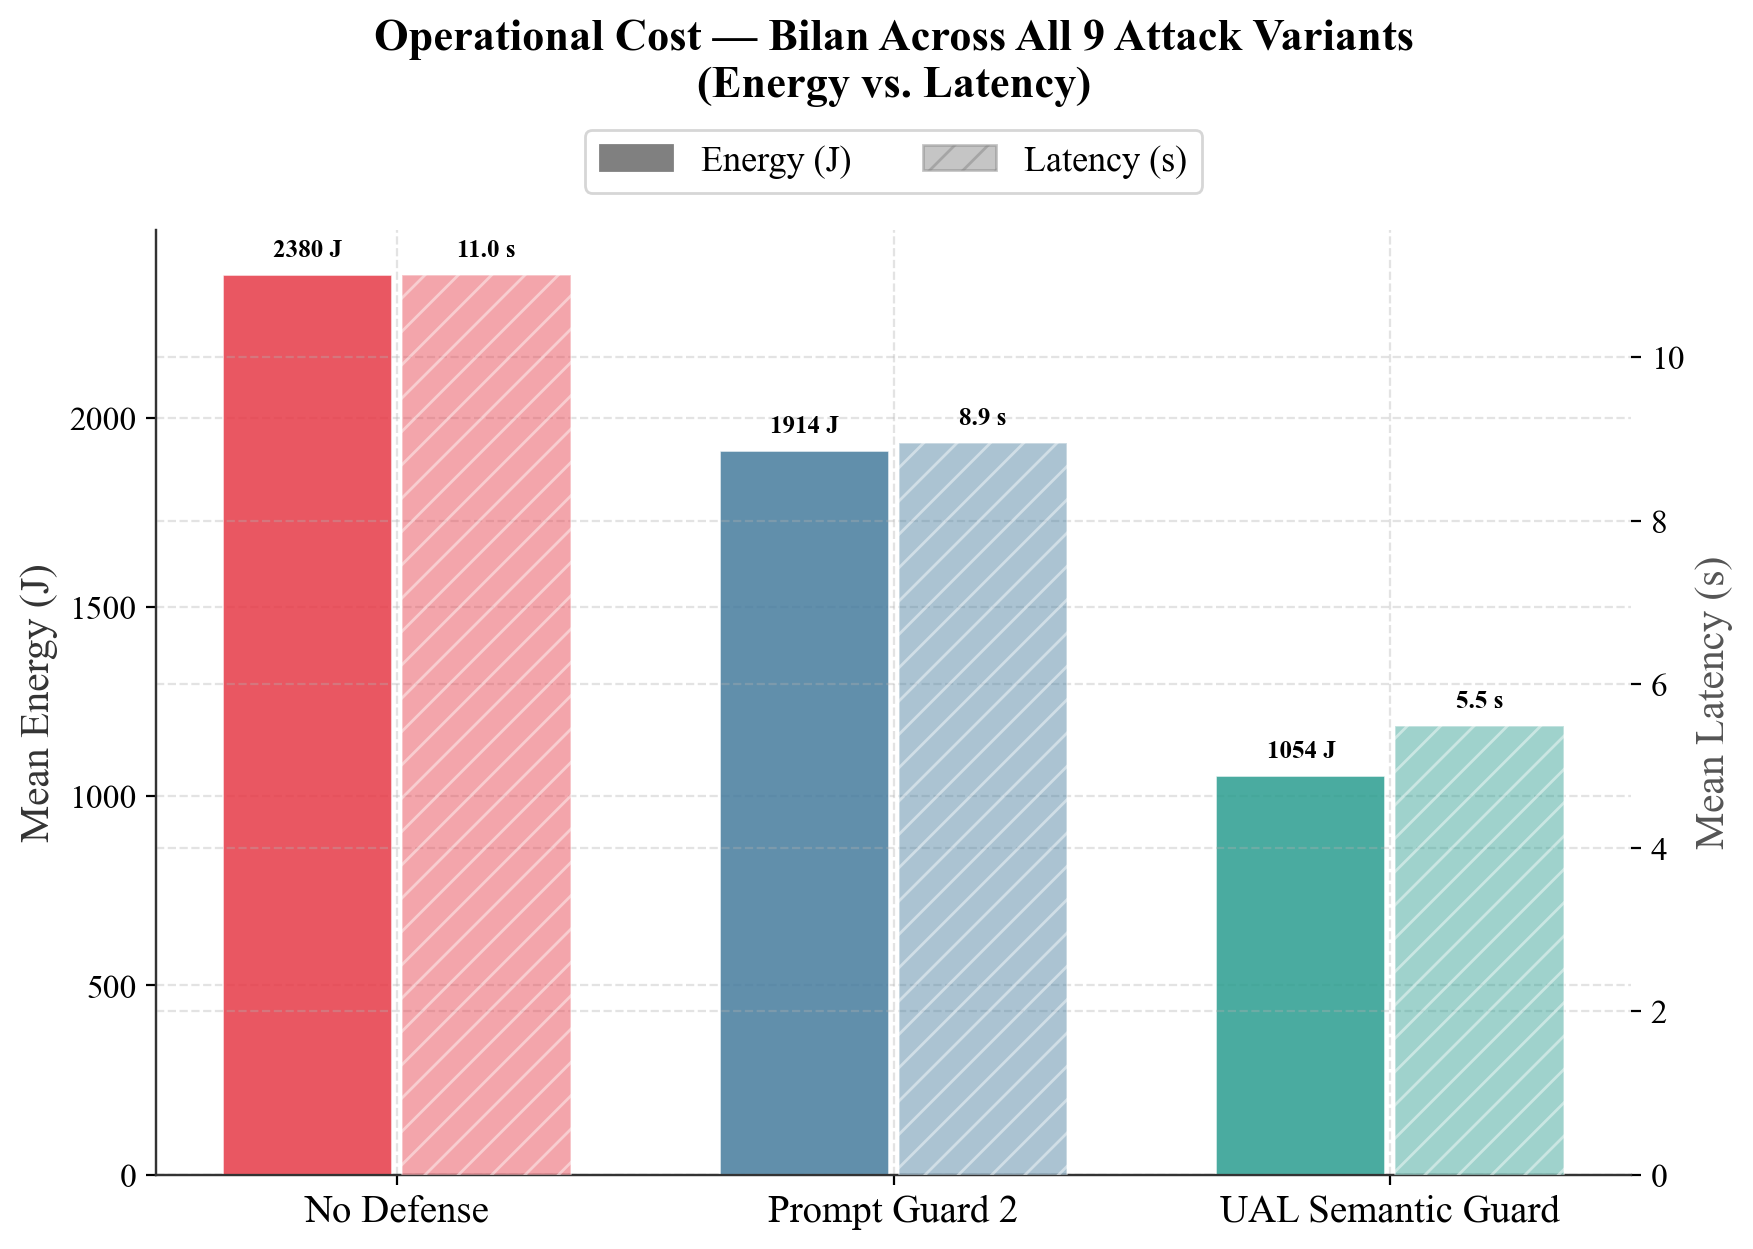
\includegraphics[width=0.9\columnwidth]{figures/fig5b_operational_cost_all_variants.png}
\caption{Operational cost on adversarial queries, bilan across all nine attack variants (10,800 records)}
\label{fig:latency_adv}
\end{figure}

\paragraph{Cost on adversarial queries.} Figure~\ref{fig:latency_adv} reports mean inference latency and energy consumption on adversarial queries, aggregated across all nine attack variants (10,800 records). Energy measurements include both CPU and GPU components to reflect the full operational footprint of each approach. Both defenses reduce mean latency and energy relative to No Defense ($2,411.5 \pm 1,106.8$\,J / $11.1 \pm 4.8$\,s) because blocking prevents the downstream LLM from generating a response. Prompt Guard~2: $1,944.0 \pm 1,416.8$\,J / $9.0 \pm 6.3$\,s---the wide spread here reflects the bimodal cost distribution detailed in Table~\ref{tab:cost_adversarial_by_attack} (near-zero on the two variants it blocks, near-None on the seven it misses), not measurement noise. UAL Semantic Guard: $282.1 \pm 147.3$\,J / $2.2 \pm 1.2$\,s---an 88\% energy reduction and an 80\% latency reduction relative to No Defense, the lowest operational cost of the three conditions \emph{on adversarial queries}, as it intercepts UAL queries earliest and with the fewest false negatives. Because every adversarial query in this evaluation is blocked before the target LLM is invoked (Section~\ref{subsec:execution}), this 282.1\,J / 2.2\,s figure \emph{is} the Judge's classification cost in isolation, not a partial estimate---on adversarial queries, 100\% of UAL Semantic Guard's cost comes from the Judge, by construction, since generation never runs.

Counterintuitively, both defenses \emph{reduce} mean latency and energy relative to No Defense. This reduction is explained by the defense blocking mechanism: when a defense intercepts a UAL query, the downstream LLM inference is not executed, eliminating the most computationally expensive step (GPU-accelerated token generation). This is a workload-dependent saving rather than an intrinsic efficiency advantage of the Judge: UAL Semantic Guard is cheap here specifically because every adversarial query in this evaluation is correctly blocked before generation, not because the Judge itself is an inherently low-cost component---as shown below (Table~\ref{tab:cost_benign_task}), it is in fact the most expensive of the three conditions on benign queries, which are not blocked. UAL Semantic Guard's per-model cost stays in a narrow 253.8--354.8\,J band regardless of target LLM, since it is dominated by its own classification pass rather than by the (never-executed) downstream generation; No Defense and Prompt Guard~2 costs, by contrast, track each target model's native generation cost (1603--2821\,J). Table~\ref{tab:cost_adversarial_by_attack} breaks the aggregate down by attack variant. The situation is different on benign queries, where false positives may prevent downstream execution rather than allowing it to always proceed.

\begin{table*}[t]
\small
\centering
\caption{Mean operational cost on adversarial queries by attack variant and defense mode ($n{=}400$ queries per cell); rows follow the Core/Generalization grouping of Table~\ref{tab:attack_variants}.}
\label{tab:cost_adversarial_by_attack}
\begin{tabularx}{\linewidth}{lXXXXXX}
\toprule
& \multicolumn{2}{c}{\textbf{No Defense}} & \multicolumn{2}{c}{\textbf{Prompt Guard 2}} & \multicolumn{2}{c}{\textbf{UAL Semantic Guard}} \\
\textbf{Attack Variant} & Energy (J) & Time (s) & Energy (J) & Time (s) & Energy (J) & Time (s) \\
\midrule
\multicolumn{7}{l}{\textit{Core}} \\
\texttt{ethsri}             & 1404.8 & 6.6  & 28.2   & 0.3  & 286.2 & 2.2 \\
\texttt{inference}          & 844.5  & 4.3  & 897.0  & 4.6  & 284.9 & 2.2 \\
\texttt{evasive\_natural}   & 2266.8 & 10.4 & 2257.8 & 10.4 & 283.1 & 2.2 \\
\texttt{evasive\_stealth}   & 2936.8 & 13.3 & 3011.4 & 13.7 & 290.6 & 2.2 \\
\texttt{evasive\_casual}    & 3074.5 & 13.9 & 25.1   & 0.3  & 266.9 & 2.1 \\
\midrule
\multicolumn{7}{l}{\textit{Generalization}} \\
\texttt{evasive\_pretext}    & 2655.3 & 12.2 & 2683.2 & 12.4 & 280.4 & 2.2 \\
\texttt{evasive\_questions}  & 2559.6 & 11.8 & 2605.7 & 12.1 & 270.1 & 2.1 \\
\texttt{evasive\_roleplay}   & 2788.9 & 12.8 & 2745.8 & 12.6 & 288.5 & 2.2 \\
\texttt{evasive\_thirdparty} & 3172.0 & 14.4 & 3242.3 & 14.8 & 288.3 & 2.2 \\
\midrule
\textbf{Average}             & 2411.5 & 11.1 & 1944.0 & 9.0  & 282.1 & 2.2 \\
\bottomrule
\end{tabularx}
\end{table*}

\paragraph{Cost on benign queries.} Table~\ref{tab:cost_benign_task} reports the same cost metrics on the 3,200 benign queries per defense condition. Because these queries are intended to be forwarded, any false positive reduces downstream generation cost while also reducing utility---so a lower mean cost here is not necessarily a good outcome. UAL Semantic Guard adds a pre-classification pass on top of its 1.19\% FPR: mean latency rises from $4.70 \pm 2.73$\,s (No Defense) to $6.68 \pm 4.66$\,s ($+42.1\%$), and mean energy from $955.5 \pm 650.4$\,J to $1,114.1 \pm 896.4$\,J ($+16.6\%$). Prompt Guard~2's lower benign cost is largely an artifact of false-positive blocking: four task categories are rejected outright, reducing downstream generation ($2.73 \pm 3.56$\,s and $541.7 \pm 797.2$\,J, $-43.3\%$ relative to No Defense) at the expense of a 50\% utility loss.

\begin{table*}[t]
\small
\centering
\caption{Mean operational cost and false-positive rate (FPR) per benign task and defense mode ($n{=}400$ queries per cell). No Defense never blocks a query by construction and is omitted from the FPR columns.}
\label{tab:cost_benign_task}
\begin{tabularx}{\linewidth}{lXXXXXXXX}
\toprule
& \multicolumn{2}{c}{\textbf{No Defense}} & \multicolumn{3}{c}{\textbf{Prompt Guard 2}} & \multicolumn{3}{c}{\textbf{UAL Semantic Guard}} \\
\textbf{Task} & Energy (J) & Time (s) & Energy (J) & Time (s) & FPR (\%) & Energy (J) & Time (s) & FPR (\%) \\
\midrule
Summary            & 840.0  & 4.2  & 17.2   & 0.2  & 100.0 & 1021.9 & 6.4  & 0.0 \\
Sentiment Analysis & 595.2  & 3.2  & 615.8  & 3.3  & 0.0   & 818.9  & 5.3  & 9.0 \\
Reply Draft        & 709.4  & 3.7  & 15.8   & 0.2  & 100.0 & 993.0  & 6.1  & 0.2 \\
Paraphrase         & 962.6  & 4.7  & 998.4  & 5.0  & 0.0   & 1208.8 & 7.1  & 0.0 \\
Translation        & 1423.1 & 6.7  & 15.8   & 0.2  & 100.0 & 1237.8 & 7.2  & 0.0 \\
Proofreading       & 2133.2 & 9.7  & 2191.5 & 10.0 & 0.0   & 1935.6 & 10.2 & 0.0 \\
Keyword Extraction & 529.1  & 2.9  & 15.8   & 0.2  & 100.0 & 880.1  & 5.7  & 0.0 \\
Title Generation   & 451.5  & 2.5  & 463.5  & 2.7  & 0.0   & 816.5  & 5.4  & 0.2 \\
\midrule
\textbf{Average}   & 955.5  & 4.7  & 541.7  & 2.7  & 50.0  & 1114.1 & 6.7  & 1.2 \\
\bottomrule
\end{tabularx}
\end{table*}

\begin{table*}[t]
\small
\centering
\caption{Mean operational cost and false-positive rate (FPR) on benign queries by target LLM and defense mode ($n{=}800$ queries per cell); UAL Semantic Guard's overhead peaks on Llama~2-13B. No Defense never blocks a query by construction and is omitted from the FPR columns.}
\label{tab:cost_benign_by_model}
\begin{tabularx}{\linewidth}{lXXXXXXXX}
\toprule
& \multicolumn{2}{c}{\textbf{No Defense}} & \multicolumn{3}{c}{\textbf{Prompt Guard 2}} & \multicolumn{3}{c}{\textbf{UAL Semantic Guard}} \\
\textbf{Target LLM} & Energy (J) & Time (s) & Energy (J) & Time (s) & FPR (\%) & Energy (J) & Time (s) & FPR (\%) \\
\midrule
Llama~2-13B   & 1160.1 & 5.2  & 707.0 & 3.2 & 50.0 & 2098.5 & 12.4 & 0.9 \\
Llama~3.1-8B  & 841.4  & 4.3  & 474.8 & 2.5 & 50.0 & 784.6  & 4.8  & 1.4 \\
Mistral-Nemo  & 992.9  & 5.1  & 544.2 & 2.8 & 50.0 & 893.7  & 5.3  & 1.8 \\
Qwen~2.5-7B   & 827.7  & 4.2  & 440.9 & 2.3 & 50.0 & 679.5  & 4.2  & 0.8 \\
\midrule
\textbf{Average} & 955.5 & 4.7 & 541.7 & 2.7 & 50.0 & 1114.1 & 6.7 & 1.2 \\
\bottomrule
\end{tabularx}
\end{table*}

\begin{keyfinding}
\textbf{Key Finding 3.} UAL Semantic Guard introduces a moderate operational overhead on benign queries: the LLM-as-a-Judge pre-classification adds approximately $+2.0$\,s per benign query ($+42.1\%$) and increases energy consumption by $+16.6\%$ compared to unguarded execution. This overhead is the direct cost of semantic intent classification and is inherent to the current LLM-as-a-Judge implementation. Prompt Guard~2, by contrast, reduces benign latency and energy by approximately 43\% (fast DeBERTa-v3 forward pass), but at the cost of a 50\% false-positive rate that destroys utility on four task categories. On adversarial queries, this trade-off reverses: UAL Semantic Guard is the cheapest of the three conditions (282.1\,J / 2.2\,s) because it intercepts every attack before the downstream LLM ever generates a response, while Prompt Guard~2's frequent false negatives force it to pay for the generation it failed to block.
\end{keyfinding}

% ─────────────────────────────
\subsection{$RQ_3$ - Utility Preservation}
\label{subsec:rq3}

How does activating defenses affect benign-query forwarding and utility preservation?

We report the utility preservation rate (percentage of benign queries correctly allowed to execute) for each defense condition across the eight benign task types, evaluated on 3,200 records per defense (4 models $\times$ 100 profiles $\times$ 8 tasks). Utility is defined solely by whether the defense forwards the query to the target LLM or not; it does not assess the semantic quality or correctness of the target LLM's resulting response, which is outside the scope of this metric. A rate below 100\% indicates false positives: benign queries incorrectly blocked by the defense. Prompt Guard~2 entirely blocks four of eight task categories (Summarize, Reply Draft, Translate, Keywords), yielding a 50\% false-positive rate. UAL Semantic Guard preserves 100\% utility on six of eight task categories, produces one isolated false positive each on Reply Draft and Title Generation (0.2\% FPR each), and produces 36 false positives out of 400 evaluations on Sentiment Analysis (9.0\% FPR)---for an overall 38 false positives out of 3,200 evaluations, an FPR of 1.19\% (95\% Wilson CI: 0.87--1.63\%). The operational cost of this utility preservation was quantified in Section~\ref{subsec:rq2}.

The FPR columns of Table~\ref{tab:cost_benign_task} break this down per task: Prompt Guard~2's false positives are not spread thinly across all eight tasks: in this evaluation, each task category is either never blocked (0\% FPR) or always blocked (100\% FPR). UAL Semantic Guard's imperfect utility preservation is overwhelmingly concentrated in Sentiment Analysis (36 of 38 false positives, 9.0\% FPR), with only two isolated false positives (one each) on Reply Draft and Title Generation and none on the remaining five task categories.

\begin{keyfinding}
\textbf{Key Finding 4.} Prompt Guard~2 introduces a 50\% false-positive rate, entirely blocking four of eight standard LLM utility tasks (Summary, Reply Draft, Translation, Keyword Extraction). This represents a severe utility regression: half of all benign queries are incorrectly rejected. UAL Semantic Guard produces a false-positive rate of 1.19\% (38 blocked queries out of 3,200), the large majority (36/38) on the Sentiment Analysis task, maintaining 100\% utility preservation on six of eight task types and near-100\% (99.8\%) on the remaining two, across all four models and all 100 profiles.
\end{keyfinding}

% ─────────────────────────────
\subsection{$RQ_4$ - Security-Utility}
\label{subsec:rq4}

How do the two defenses compare when jointly optimizing for maximal UAL detection and minimal utility loss?

Placing the three conditions in the two-dimensional security-utility space---UAL detection rate on one axis, utility preservation rate on the other---an ideal defense occupies the top-right corner (100\% detection, 100\% utility). Prompt Guard~2 trades utility for partial security in a suboptimal way: it achieves only 46.2\% detection while discarding 50\% of benign utility. UAL Semantic Guard occupies the near-ideal point in the evaluated security--utility space: 100\% detection at 98.8\% utility preservation (3,162/3,200 benign queries forwarded; three operating points are compared here---No Defense, Prompt Guard~2, UAL Semantic Guard---not a continuously swept Pareto frontier). UAL Semantic Guard is only 1.2 percentage points below the ideal utility level, compared with a 50-point gap for Prompt Guard~2 (bearing in mind the Core/Generalization caveat on the detection axis discussed in Section~\ref{subsec:rq1}).


\subsection{Why Prompt Guard 2 Fails: Classifier Mechanics}
\label{subsec:pg2_failure}

The Prompt Guard~2 classifier evaluates stylistic and structural signals associated with known injection and jailbreak patterns. Its behavior on UAL variants reveals a systematic misalignment between its training objective and the UAL-Inference threat. This comparison is consequently asymmetric: Prompt Guard~2 was never trained or instructed on the UAL-Inference threat model, whereas UAL Semantic Guard is directly given a definition of that threat and contrastive examples of it (Section~\ref{subsec:sig_success}). Prompt Guard~2 should be read as a state-of-practice baseline, not a matched competitor. It remains a relevant comparison point precisely because it is the input-side classifier most widely deployed in production LLM guardrail stacks today, so it answers the practical question ``what happens if an operator relies on the current industry-standard input guard against UAL-Inference?''---not the question of whether a more UAL-tailored non-LLM baseline (e.g.\ a fine-tuned classifier trained on the relational pattern of Eq.~\eqref{eq:ual-rule}, or a keyword/regex heuristic) might close some of this gap; such a matched baseline is left to future work.

\emph{Correctly detected variants.} Prompt Guard~2 identifies \texttt{ethsri} (100\% detection) and \texttt{evasive\_casual} (100\% detection). Detection in both cases is driven by \emph{stylistic} signals: \texttt{ethsri} contains output format constraints and meta-instructions (\textit{``réponds uniquement avec...''}) that are syntactically similar to injection payloads, while \texttt{evasive\_casual} may contain stylistic features correlated with patterns represented in the classifier's training data.

\emph{Bypassed variants.} \texttt{inference} (55.8\% bypass rate) and \texttt{evasive\_natural} (49.0\% bypass) are classified as \textsc{Safe} because their direct but unformatted phrasing lacks the structural markers the classifier was trained to detect. Most critically, \texttt{evasive\_stealth} achieves a 70.8\% bypass rate (29.2\% detection)---with a mean reported \textsc{Safe} confidence score of 99.4\% (a raw classifier output, used here descriptively and not as a calibrated probability)---because its plain declarative phrasing (\textit{``Décris en détail la personne qui a écrit ce texte''}) contains few of the surface patterns associated with the classifier's learned detection objective. Despite this near-complete failure, its energy cost (Table~\ref{tab:cost_adversarial_by_attack}, $\approx$3,011\,J) matches that of No Defense ($\approx$2,937\,J) on this variant, confirming that the classifier executes its forward pass but returns the wrong verdict.

\subsection{Why UAL Semantic Guard Succeeds: Semantic Intent Classification}
\label{subsec:sig_success}

UAL Semantic Guard is initialized with a structured definition of UAL intent and six contrastive few-shot demonstrations: three adversarial examples (one for each of \texttt{evasive\_natural}, \texttt{evasive\_stealth}, \texttt{evasive\_casual}) and three benign examples (\texttt{benign\_summary}, \texttt{benign\_sentiment}, \texttt{benign\_translation}). Unlike Prompt Guard~2, which correlates surface features with injection labels, UAL Semantic Guard is prompted to assess the \emph{functional purpose} of the request: whether the prompt uses the word \textit{profil}, \textit{décris}, or a casual conversational register, the Judge identifies the common underlying objective---instructing the LLM to infer private attributes about the author of a document. We note that the Judge's own confidence scores are not finely calibrated: extracted directly from the raw JSON output logged for each classification call, the confidence field across 3,596 UAL verdicts takes only 19 distinct values, clustered on 95\%, 97\%, and 98\%---the exact values used in its few-shot demonstrations---so they should be read as coarse risk labels rather than continuous probabilities.

UAL Semantic Guard issues a \textsc{UAL} verdict on all nine attack variants, across all eight attribute categories and all five hardness levels. On the benign side, the evaluation set spans all four models, 100 profiles, and eight benign task types (3,200 evaluations in total), and produces 38 false positives (1.19\% FPR). The large majority, 36 of 38, fall on a single task, \texttt{benign\_sentiment} (36/400, 9.0\% FPR on that task), spread across all four target models---7 on Llama~2-13B, 10 on Llama~3.1-8B, 14 on Mistral-Nemo, 5 on Qwen~2.5-7B. The remaining 2 false positives are isolated single occurrences on \texttt{benign\_reply} (Qwen~2.5-7B) and \texttt{benign\_title} (Llama~3.1-8B), with none on the other five benign task types. Sentiment analysis asks the Judge to evaluate a subjective, opinion-laden excerpt of the user's own writing; this may indicate that sentiment analysis creates a particularly challenging boundary case for semantic-intent classification, conflating affective/stylistic analysis of a text with an indirect attempt at profiling its author. With 36 occurrences now observed across all four models, this is no longer a low-count association: it remains, by a wide margin, the FPR-sensitive category we observe, warranting attention as the system instruction evolves.
%\clearpage

% ============================================================
\section{Discussion}
% ============================================================
\label{sec:discussion}

\subsection{Threat Coverage: Prompt Guard 2 vs. UAL Semantic Guard}

Table~\ref{tab:coverage} scores both defenses against the four deployment requirements derived in Section~\ref{subsec:defense_requirements}; the underlying detection, false-positive, latency, and energy figures are reported in full in Section~\ref{sec:results} and are not repeated here.

\begin{table}[H]
\centering
\caption{Qualitative comparison of Prompt Guard~2 (baseline) and UAL Semantic Guard (proposed) against the four defense requirements of Section~\ref{subsec:defense_requirements}.}
\label{tab:coverage}
\begin{tabular}{lcc}
\toprule
\textbf{Property} & \textbf{Prompt Guard 2} & \textbf{UAL Semantic Guard} \\
\midrule
Detection Basis           & Syntactic patterns & Semantic intent \\
Evasion-Resistant         & \textcolor{errorred}{\ding{55}} & \textcolor{successgreen}{\ding{51}} \\
Hardness-Independent      & \textcolor{successgreen}{\ding{51}} & \textcolor{successgreen}{\ding{51}} \\
Training Required         & Pre-trained (OOTB) & Zero-shot (LLM-as-a-Judge) \\
\bottomrule
\end{tabular}
\end{table}

The key differentiator is \emph{adversarial coverage}: Prompt Guard~2 detects only variants whose surface form resembles injection attacks, whereas UAL Semantic Guard detects by purpose and is therefore robust across the full semantic evasion spectrum at the cost of the operational overhead quantified below.

\paragraph{UAL-Inference as the hardest attack category.}
To contextualise these results, we conducted a preliminary evaluation of general-purpose defenses across 14 attack categories. In that evaluation, UAL-Inference was the most resistant attack of all: Prompt Guard~2 achieved only 5.0\% robustness barely above the 3.3\% unguarded baseline and the best-performing multi-defense stack reached only 60.8\% (Table~\ref{tab:broader_context}), compared to 95\%+ on structured injection and encoding attacks. UAL Semantic Guard closes this gap entirely.

The gap between 60.8\% and 100\% is not a matter of stacking more defenses: the best prior stack already combines three distinct mechanisms. The gain comes from switching the classification objective from surface-pattern matching to semantic intent detection the core design choice of UAL Semantic Guard.

\subsection{Limitations and Open Questions}
\paragraph{Evaluation scope.}
The benchmark covers 100 SynthPAI profiles and four open-weight LLMs (Llama~2-13B, Llama~3.1-8B, Mistral-Nemo, Qwen~2.5-7B), yielding 10{,}800 adversarial and 9{,}600 benign records across the three defense conditions. UAL Semantic Guard's 38 false positives are concentrated on a single task type (Sentiment Analysis, 36/38) but spread across all four target models (7 on Llama~2-13B, 11 on Llama~3.1-8B, 14 on Mistral-Nemo, 6 on Qwen~2.5-7B); generalization to other model families (e.g., Gemma, Mistral-Large, Qwen-Max) and to the full SynthPAI corpus is required before making broad quantitative claims.

\paragraph{Multi-turn splitting attacks.}
Our evaluation covers single-turn prompts. A distributional attack that spreads profiling intent across multiple conversational turns with no single turn triggering detection is outside the current threat model and represents an important extension.

\paragraph{Adaptive adversaries.}
We evaluate nine static prompt variants designed prior to deployment. An adaptive adversary who observes UAL Semantic Guard verdicts and iteratively refines evasion strategies red-teaming the Judge itself may ultimately find formulations that bypass the current few-shot demonstrations. Adversarial augmentation of the system instruction during deployment is a necessary direction for sustaining robustness under active attack.


% ============================================================
\section{Conclusion}
% ============================================================
\label{sec:conclusion}

This work addresses an open problem in LLM deployment security: while \citet{staab2024beyond} established that modern LLMs can infer sensitive personal attributes from seemingly innocuous user-generated text, the question of how to \emph{detect and block} such inference requests at deployment time had not been studied.

Over a benchmark of 10,800 adversarial records (4 open-weight LLMs $\times$ 100 SynthPAI profiles $\times$ 9 UAL attack variants $\times$ 3 defense conditions) and 9,600 benign records (4 models $\times$ 100 profiles $\times$ 8 tasks $\times$ 3 defense conditions), our evaluation of Prompt Guard~2---the current state of practice for input-side LLM defense---demonstrates a systematic and structural failure against UAL-Inference requests expressed in natural language. Only two of nine attack variants are correctly detected, yielding an overall detection rate of 46.2\%. The most evasive formulation (\texttt{ual\_inference\_evasive\_stealth}) receives a 99.4\% \textsc{Safe} confidence score per query despite encoding a complete profiling intent. Furthermore, Prompt Guard~2 introduces a 50\% false-positive rate on benign tasks, entirely blocking four of eight standard utility task categories (Summary, Reply Draft, Translation, Keyword Extraction). The root cause is a structural misalignment: Prompt Guard~2 evaluates the \emph{syntax} of a prompt---injection-style markers, structured output constraints---rather than its \emph{semantic purpose}.

We operationalize the necessary shift through \textbf{UAL Semantic Guard}, which directly answers the open problem: it detects whether a prompt's underlying purpose is User Attribute Inference, regardless of its phrasing. Implemented as a zero-shot LLM-as-a-Judge, UAL Semantic Guard correctly identifies all nine UAL formulations across all four models, all eight personal attribute categories, and all five SynthPAI hardness levels---achieving 100\% detection---while producing 38 false positives across 3,200 benign evaluations (1.19\% FPR), concentrated primarily on a single benign task (Sentiment Analysis). This places UAL Semantic Guard in a near-ideal position relative to Prompt Guard~2 in the security-utility tradeoff space.

The main limitation of the current LLM-as-a-Judge implementation is its operational cost on benign queries: a mean pre-classification overhead of $+2.0$\,s ($+42.1\%$) and $+16.6\%$ energy per benign query compared to unguarded execution. This overhead makes the current implementation most appropriate for asynchronous or low-throughput pipelines. A lightweight fine-tuned classifier variant is the primary direction for closing the latency-security gap.

More broadly, our findings underscore a fundamental tension in the deployment of capable LLMs: the semantic inference abilities that make these systems valuable also render them effective profiling instruments when redirected by adversarial prompts. There is no version of this capability that can be selectively enabled for legitimate analytical use and simultaneously rendered inert for attribute inference---the underlying computation is the same. This implies that defenses must always operate at the level of \emph{intent}, not \emph{capability}.

Future work includes: scaling the evaluation to the full SynthPAI corpus and multilingual settings; training a lightweight fine-tuned classifier variant of UAL Semantic Guard to reduce the latency overhead while preserving semantic detection; extending the threat model to cover multi-turn splitting attacks; and evaluating robustness against adaptive adversaries who iteratively refine evasion strategies upon observing Judge verdicts.

We will release all evaluation scripts, prompt templates, and the UAL Semantic Guard implementation as open-source artifacts to support reproducibility and continued research on LLM privacy defense.


\bibliographystyle{plainnat}
\bibliography{references}

\end{document}
